\chapter{Optical Modelling and Design Analysis}
\label{Cap:Opt}

\section{Aims and objectives}

This chapter aims to define the design of a concentrating collector for an air heating system using ray tracing optical analysis. The specific objectives are to:

\begin{itemize}[topsep=5pt,partopsep=0pt] \itemsep0pt
%\setlength\itemsep{0pt}
	\item Develop a ray tracing technique in 3D and implement the optical model in Matlab$^{\circledR}$;
	%\item Implement an optical model algorithm in Matlab$^{\circledR}$;
	\item Evaluate the effect of the parabolic reflectors and the tertiary cavity geometry on the optical performance;
	\item Assess the impact of the concentrator's length on reflector cost;
	\item Analyse the influence of the glazing inclination on the light transmittance through the glazed aperture;
	\item Characterise the optical profile of a concentrator used for experimental tests.
	%\item Specify the proposed concentrator's design to be used in this work;
	%\item To compare the energy distribution along the absorber between 2D and 3D ray tracing model;
	%\item To validate the 2D ray tracing model with a laser test.
\end{itemize}

\section{Design considerations of the concentrator}

\subsection{Overall assembly}

The proposed solar concentrator combines an inverted absorber with an asymmetric compound parabolic concentrator (ACPC). It comprises: i) two parabolic reflectors, ii) a circular reflector, iii) two straight reflectors, iv) two end reflectors, v) a glazing cover not coincident with the aperture, and vi) a transpired absorber plate. The entire collector is oriented south. A full drawing and cross-section are shown in Figures \ref{collector3D} and \ref{CSview}, respectively. 

\Figure[scale=0.40,placement=!ht,label={collector3D},caption={Concentrator's design in 3D.}]{figs/collector3D.PNG}

\Figure[scale=0.70,placement=!ht,label={CSview},caption={Concentrator's cross-section view.}]{figs/CSview2.eps}

\subsection{Glazing position}
The glazing placed from the aperture confines heated air in the collectors and protects the collector's interior against weather conditions (\cite{Shams2016}). Its position at a given inclination $\beta$ (shown in Figure \ref{CSview}) to the horizontal plane seeks to gain solar energy transmittance and reduce light reflection.

\subsection{Aperture position}
The concentrator's aperture is set at the vertical position (at the truncation line in Figure \ref{CSview}) so that shading can be avoided when two or more collectors are stacked on a vertical wall, enabling the full fa\c{c}ade area available to be harnessed.

\subsection{Parabolic shape}
The angles of both parabolas axes ($\theta_{\!_{\rm{P1}}}$ and $\theta_{\!_{\rm{P2}}}$) shown in Figure \ref{CSview} define the parabolic shape, therefore affecting size, angular acceptance range (\cite{Zacharopoulos2000}; \cite{Harmim2012}) and maximum geometric concentration ratio (\cite{Mills1978}). Given the same concentration ratio, concentrators of narrow angular acceptance are more efficient, so they collect higher amounts of the available solar energy  (\cite{Sarmah2011}).
    
\subsection{Cavity height}
The cavity contributes to the formation of thermally stratified air layers below the absorber, suppressing convective and radiative heat losses. The height of this cavity affects the distribution of incoming solar radiation along the absorber surface to enhance the heat transfer mechanism and mitigate hot spots.

\section{Operation conditions}

This solar air heating system is designed to operate in Dublin, Ireland, where the latitude ($\phi$) is 53.35$^{\circ}$ north and the longitude is -6.26$^{\circ}$ over the summer season (from 21/06 to 21/09) for 8 hours per day, from 9 am to 5 pm (local time).

Defining the operating constraint is an essential prerequisite to calculate the Sun angles applicable to the period of operation. They are obtained using solar time ($\rm{t_{st}}$, in h), which does not coincide with the local standard time (${\rm t_{\!_{LST}}}$, in h). The relationship between solar and local times, given by Eq. (\ref{solartime}), is due to the deviation between the local longitude ${\rm \ell_{local}}$ and the chosen meridian (${\rm \ell_{st}}$) on which the local standard time is based.

\begin{equation}
    \mathrm{t_{st} = t_{\!_{LST}} + \frac{4(\ell_{st} - \ell_{local}) + E_T}{60}}
    \label{solartime}
\end{equation}

Irregularity of the earth's motion around the Sun is accounted for by the "Equation of Time" ($\rm{E_T}$, in min) as a function of the year's day (\cite{Goswami2015}). Solar hour angles ($\omega_{\rm{s}}$) were obtained from the solar time for each day of operation. 

%The solar altitude and solar azimuth angles (${\rm a_s}$ and $\gamma_{\rm{s}}$) were calculated from (\cite{Duffie2013}):
%
%\begin{equation}
%\mathrm{{a_s} = {\sin ^{ - 1}}\left( {\sin \phi \sin {\delta _s} + \cos \phi \cos {\delta _s}\cos {\omega_s}} \right)}
%\label{solar_alt}
%\end{equation}
%\vspace*{-0.5cm}
%\begin{equation}
%\mathrm{\gamma_s = {\sin^{-1}}\left(\frac{\cos \omega_s \sin \delta_s}{\cos a_s}\right)}
%\label{azimuth}
%\end{equation}
%
%\noindent where the solar declination $\delta_{\rm{s}}$ is a function of the year's day.

A solar position plot of ${\rm a_s}$ against $\gamma_{\rm{s}}$ at the latitude of Dublin is shown in Figure \ref{Alt_Azz}, where each graph corresponds to a particular day in the operation period. The values of ${\rm a_s}$ and $\gamma_{\rm{s}}$ at any point in time in the operation period were used as inputs in the optical modelling. The calculation of these solar angles was verified by Sun calculators available on the Internet (\cite{Time2018}; \cite{SunCalc2018}).

\Figure[scale=0.60,placement=!ht,label={Alt_Azz},caption={Solar position diagram for 53.35$^{\circ}$ of latitude north.}]{figs/Alt_Azz2.eps}

Throughout the operation, the calculated limits of altitude solar angle were 60.1$^{\circ}$ when the Sun is at its highest altitude, on 21/06 at noon; and 14.6$^{\circ}$ when the Sun is at its lowest altitude in the last day of summer (21/09) at 9 am. The collector must, therefore, accept direct solar radiation within the solar altitude range, from 15$^{\circ}$ to 61$^{\circ}$.

\section{Reflector's design specification}

%\subsection{Software tools used}

%This section describes how the reflectors were designed and placed to form the proposed air heating concentrator. The design was performed in Matlab$^{\circledR}$ with the help of SolidWorks$^{\circledR}$ by using positive x-y coordinates.

\subsection{Parabolic reflectors design}

To design the parabolic reflectors, the first step was to define the equation of the parabola whose axis is coincident to the y-axis with the vertex set at the origin:

\begin{equation}
\mathrm{{y} = \left( {\frac{1}{{4f}}} \right){x}^2}
\label{parabola}
\end{equation}

\noindent where x and y are the coordinates in the xy plane and f is the focal distance (m), given by Eq. (\ref{focal}) (\cite{Winston2005}):

\begin{equation}
\mathrm{f = \frac{{{W_{abs}}}}{2}\left( {1 - \cos {\theta_{a}}} \right)}
\label{focal}
\end{equation}

\noindent and $\rm{\theta_{a}}$ is the angle related to the position of the parabola and ${\rm W_{abs}}$ is the absorber width (m). The next step was translating and rotating the parabola to form the parabolic section. Both parabolas were designed and placed at the correct position using basic tools from SolidWorks$^{\circledR}$ as shown in Figure \ref{rottrans_two}. The expressions for calculating $\rm{\theta_{a}}$, $\rm{\Delta x}$ (displacement in the x-direction) and $\rm{\Delta y}$ (displacement in the y-direction) for each parabola are shown in Table \ref{parabolas}.

\begin{figure}[ht!]
	\begin{minipage}{0.49\columnwidth}
		\includegraphics[width=0.9\columnwidth,height=6.0cm]{figs/upper_parabola.PNG}
		\subcaption{Upper parabola.}
	\end{minipage}
	\begin{minipage}{0.49\columnwidth}
		\includegraphics[width=0.9\columnwidth,height=6.0cm]{figs/lower_parabola.PNG}
		\subcaption{Lower parabola.}
	\end{minipage}
	\caption{(a) Upper and (b) lower parabolas placed at the final position.}
	\label{rottrans_two}
\end{figure}

\begin{table}[!ht]
	\centering
	\caption{Expressions for the parabolas' parameters.}
	\begin{tabular}{cp{3.3cm}l}
		\hline \\[-12pt]
		\vspace*{0.1cm} Parameter & Upper Parabola & Lower Parabola \\ [0pt]
		\hline \\[-12pt]
		$\theta_{{\rm{a}}}$ & $90 -\theta_{\!_{\rm{P1}}}$ & 2$\theta_{\!_{\rm{P2}}}$ \\ [5pt]
		%$\theta_{\!_{\rm{R}}}$ & 90 $- \alpha_{\!_{\rm{P1}}}$ & 90 $- \alpha_{\!_{\rm{P2}}}$ \\ [5pt]
		$\Delta \rm{x}$ & $\rm{{W_{abs}} - f\cos {\theta_{\!_{P1}}}}$ & $\rm{{W_{abs}} - ({W_{abs}} + f)\cos {\theta_{\!_{P2}}}}$ \\ [5pt]
		$\Delta \rm{y}$ & $\rm{- f\sin {\theta_{\!_{P1}}}}$ & $\rm{({W_{abs}} - f)\sin {\theta_{\!_{P2}}}}$ \\ 
		\hline 
	\end{tabular}
	\label{parabolas}
\end{table}

\newpage
The next step was to arrange the parabolas properly in a common coordinate system to form the full untruncated parabolic section shape APQD, shown in Figure \ref{twoparabolas22}. In this case, point D intercepts the x-axis and the vertical segment length AD equals $\rm{W_{abs}}$, the section end. The full aperture indicated by the segment PQ is obtained according to the angles of the parabola axes. The aperture was set to be vertical; therefore, the section is truncated at the line indicated by segment BC. The AB and DC curves represent the shapes of the upper and lower reflectors, respectively. Their coordinate limits are given in Table \ref{coordinates}.

\Figure[scale=0.55,placement=!ht,label={twoparabolas22},caption={Two parabolas arranged to form the truncated parabolic section (ABCD). Dashed curves of the parabolas were eliminated.},shortcaption={Two parabolas assembled to form the truncated parabolic section (ABCD)}]{figs/fig_primary3.PNG}

\begin{table}[!ht]
	\centering
	\caption{Reflector coordinate limits.}
	\begin{tabular}{lll}
		\hline \\[-12pt]
		\vspace*{0.1cm} Reflector & x limits & y limits \\ [0pt]
		\hline \\[-12pt]
		Upper & $\rm{{W_{abs}} \le {x} \le {x_{apt}}}$ & $\rm{{W_{abs}} \le {y} \le {y_{apt,upper}}}$ \\ [5pt]
		Lower & $\rm{{W_{abs}} \le {x} \le {x_{apt}}}$ & $\rm{0 \le {y} \le {y_{apt,lower}}}$ \\ 
		\hline 
	\end{tabular}
	\label{coordinates}
\end{table}

%The mathematical process of rotation and translation was achieved using the Affine transformation technique (\cite{Duffy2016}), which consists of applying a matrix multiplication as shown in Eq. (\ref{affine}):
%
%\begin{equation}
%\left[ {\begin{array}{*{20}{c}}
%		\mathrm{{{x }}}\\
%		\mathrm{{{y }}}\\
%		1
%		\end{array}} \right] = \left[ {\begin{array}{*{20}{c}}
%		1&0&\mathrm{\Delta x}\\
%		0&1&\mathrm{\Delta y}\\
%		0&0&1
%		\end{array}} \right]\left[ {\begin{array}{*{20}{c}}
%		\mathrm{\cos {\theta_{\!_R}}}&\mathrm{\sin {\theta_{\!_R}}}&0\\
%		\mathrm{- \sin {\theta_{\!_R}}}&\mathrm{\cos {\theta_{\!_R}}}&0\\
%		0&0&1
%		\end{array}} \right]\left[ {\begin{array}{*{20}{c}}
%		\mathrm{{{ x_p }}}\\
%		\mathrm{{{ y_p }}}\\
%		1
%		\end{array}} \right]
%\label{affine}
%\end{equation}
%
%\noindent with the parameters $\rm{\Delta x}$ and $\rm{\Delta y}$ as the displacements in x and y, respectively, $\rm{\theta_{\!_R}}$ as the angle of rotation (which is the complement of the parabola axis angle), and $\rm{{{x}}}$ and $\rm{{{y}}}$ are the new coordinates of the parabola calculated by the Affine transformation technique. 
%
%The mathematical equation to represent a rotated-translated parabola is implicit defined by an irreducible polynomial of second degree, which is complex solve for ray tracing applications. Another way of representing the portion of the parabolic reflectors was thus used to approximate the parabolic shapes to a $\rm{N_d}^{\rm{th}}$ degree polynomial fit  in the form of:
%
%\begin{equation}
%\mathrm{y = \sum\limits_{j = 0}^{N_d} {{a_j}x^j}}
%\label{eqP1}
%\end{equation}
%
%\noindent where the linear coefficients $\rm{a_{\!_{0}}}$, $\rm{a_{\!_{1}}}$, $\rm{a_{\!_{2}}}$, $\rm{a_{\!_{3}}}$, ..., $\rm{a_{\!_{Nd}}}$ and the degree order $\rm{N_d}$ were determined in a way to maximise the fit using a linear least-squares solver with linear constraints.

The equations used to model the parabolas consider x and y as functions of a new parametric variable $\rm{t_p}$ assigned for each parabolic shape, as shown in Eqs. (\ref{p_x}) and (\ref{p_y}). These parametric equations model the exact parabolic shapes and are quadratic polynomials in $\rm{t_p}$, which takes minimum process time to be solved. 

\begin{equation}
	\mathrm{x = \frac{1}{4f}\sin\theta_a t_{p}^2 + \cos\theta_a t_p + \Delta x}
	\label{p_x}
\end{equation}
\vspace*{-0.75cm}
\begin{equation}
	\mathrm{y = \frac{1}{4f}\cos\theta_a t_{p}^2 - \sin\theta_a t_p + \Delta y}
	\label{p_y}
\end{equation}

\noindent where the parametric variables range to provide x and y coordinates whose limits are established in Table \ref{coordinates}.

\subsection{Circular reflector design}

A quarter of a circle was used for the circular reflector, whose centre was set at \mbox{($\rm{W_{abs}}$, $\rm{W_{abs}}$)} and radius $\rm{W_{abs}}$. Eq. (\ref{quartercircle}) expresses the calculation for the circular section:

\begin{equation}
	\mathrm{{y} = {W_{abs}} - \sqrt {\mathrm{W_{abs}^2 - {{\left( {{x} - {W_{abs}}} \right)}^2}}}}
	\label{quartercircle}
\end{equation}

\noindent where the coordinate limits are $\rm{0 \le {x} \le {W_{abs}}}$ and $\rm{0 \le {y} \le {W_{abs}}}$. The shape of the circular sector is illustrated in Figure \ref{three_sections} by the curve DE. 

\subsection{Straight reflector design}

The straight reflector section comprises two vertically straight reflectors of height $\rm{H_{\!_{TS}}}$ above the circular section and ends at the absorber surface (whose y-coordinate is $\rm{y_{\!_{TS}}}$). The coordinate limits here are $\rm{0 \le {x} \le {W_{abs}}}$ and $\rm{W_{abs} \le {y} \le {y_{\!_{TS}}}}$. Figure \ref{three_sections} represents them by the vertical segments EF and AG.
%, as shown in Figure \ref{TS_SS}.

\subsection{End reflectors design}

The end reflectors are two identical flat surfaces, one at each end of the concentrator (west and east sides shown in Figure \ref{collector3D}), where their boundaries are the shapes of the other reflectors.

\subsection{Summary of overall coordinates}

Figure \ref{three_sections} illustrates all the reflectors arranged along with the main coordinates.

\Figure[scale=0.35,placement=!ht,label={three_sections},caption={Concentrator's cross-section view with the appropriate coordinate information.}]{figs/three_sections.PNG}

Figure \ref{three_sections3D} shows the concentrator in three dimensions where:

\begin{itemize}[topsep=5pt,partopsep=0pt] \itemsep0pt
\item AHIB and DKJC are the upper and lower parabolic reflectors;
\item ELKD is the circular reflector;
%\item ELMF and AHNG are the straight reflectors;
\item ABCDEFG and HIJKLMN are the western and eastern end reflectors, respectively;
\item FMNG is the absorber surface and BIJC is the aperture;
\item The concentrator’s main dimensions are: depth $\rm{W_{col}}$, height $\rm{H_{col}}$ and length $\rm{L_{col}}$.
\end{itemize}

\Figure[scale=0.55,placement=!ht,label={three_sections3D},caption={Final concentrator concept.}]{figs/collector3D-3.PNG}

\section{Ray Tracing and Optical Modelling}

The complex geometry of the IACPC makes it difficult to predict its optical performance with analytical equations. To overcome this challenge, a 3D ray tracing algorithm in Matlab was used to simulate direct solar radiation entering through the aperture, reflecting off the reflectors, and reaching the absorber. Figure \ref{triad} illustrates a 3D coordinate system used to represent the geometry of a ray in space. It defines a vector with its initial point $\rm{(x_0, y_0, z_0)}$ from which the ray originates and a point of incidence $\rm{(x_{\text{int}}, y_{\text{int}}, z_{\text{int}})}$ where the ray intersects the surface. It is also defined by its angular components  $\theta_{iy}$ and  $\theta_{iz}$. The diagram describes a ray's spatial orientation in the system's context.

\begin{figure}[!ht]
	\centering
	\begin{tikzpicture}[scale=5,tdplot_main_coords,very thick,framed]
		\coordinate (O) at (0,0,0);
		\tdplotsetcoord{P}{\rvec}{\thetavec}{\phivec};
		\draw[arrow] (0,0,0) -- (0.75,0,0) node[anchor=north east]{x (south)};
		\draw[arrow] (0,0,0) -- (0,0.75,0) node[anchor=north west]{z (east)};
		\draw[arrow] (0,0,0) -- (0,0,0.75) node[anchor=south]{y (up)};
		\draw[arrow,color=red] (P) node[anchor=west]{\color{black}Initial point ($\rm{x_0,y_0,z_0}$)} -- (O) node[anchor=east]{\color{black}Point of incidence ($\rm{x_{int},y_{int},z_{int}}$)};
		\draw[dashed, color=red] (O) -- (Pxy);
		\draw[dashed, color=red] (P) -- (Pxy);
		\tdplotdrawarc{(O)}{0.2}{0}{\phivec}{anchor=north}{$\rm{\theta_{iz}}$}
		\tdplotsetthetaplanecoords{\phivec}
		\tdplotdrawarc[tdplot_rotated_coords]{(O)}{0.25}{90}{\thetavec}{anchor= south west}{$\rm{\theta_{iy}}$}
	\end{tikzpicture}
	\caption{Orientation in 3D of one incoming ray going through the concentrator.}
	\label{triad}
\end{figure}

The flowchart in Figure \ref{flow-opt} outlines how to trace a ray through the concentrator and determine its optical efficiency. The process begins by defining the concentrator's boundaries and initialising the ray's path. As the ray is traced, intersections with the concentrator's reflectors -- such as the ends, parabolic surfaces, and straight segments -- are checked. Each intersection adds a reflection to the ray's path. The total number of reflections is summed if the ray reaches the absorber, and the optical efficiency is determined. If the ray fails to reach the absorber, it is rejected, and the optical efficiency is set to zero. The process ends when the efficiency is calculated, or the ray is rejected.

%\singlespacing
\begin{figure}[!ht]
	\centering
	\scalebox{0.8}[0.8]{
		\begin{tikzpicture}[node distance = 3cm]
			\node[startstop,xshift=-1cm] (start) {Start};
			\node[input, right of=start,text width=6cm] (init) {Build concentrator's boundaries; Build initial ray's line equation};
			\node[block, below of=init, text width=4cm,yshift=1.5cm,text width=2.5cm] (new) {Start ray};
			\node[decision, below of =new,yshift=0.75cm] (rend) {Intersection w/ either end?};
			\node[decision, below of = rend,yshift=-1cm,text width = 2.25cm] (rupper) {Intersection w/ upper parabolic?};
			\node[decision, below of = rupper,yshift=-1cm,text width = 2.25cm] (rlower) {Intersection w/ lower parabolic?};
			\node[decision, below of = rlower,yshift=-1cm,text width = 2.25cm] (rcirc) {Intersection w/ circular?};
			\node[decision, below of = rcirc,yshift=-1cm,text width = 2.25cm] (rstr) {Intersection w/ either straight?};
			\node[decision, right of = rstr,xshift=1.5cm] (abs) {Ray reaching the absorber?};
			\node[block, right of=abs,xshift=2cm,text width=3.5cm] (calc) {Get total number of reflections and calculate optical efficiency};
			\node[startstop,below of=calc,yshift=-1.25cm] (end) {End};
			\node[block, below of=abs,yshift=-1.25cm,text width=4cm] (rej) {This ray is rejected; Optical efficiency = 0};
			
			\draw[arrow] (start) -- (init);
			\draw[arrow] (init) -- (new);
			\draw[arrow] (new) -- coordinate[midway](m1)(rend);
			\node[block, left of=m1,xshift=-1cm] (ref) {Add one reflection};
			\draw[arrow] (ref) -- (m1);
			\draw[arrow] (rend) -| coordinate[pos=0.1](m2) (ref); \node [black,above=0.01 of m2] {Yes};
			\draw[arrow] (rend) -- node[anchor=east] {No} (rupper);
			\draw[arrow] (rupper) -| coordinate[pos=0.1](m3) (ref); \node [black,above=0.01 of m3] {Yes};
			\draw[arrow] (rupper) -- node[anchor=east] {No} (rlower);
			\draw[arrow] (rlower) -| coordinate[pos=0.1](m4) (ref); \node [black,above=0.01 of m4] {Yes};
			\draw[arrow] (rlower) -- node[anchor=east] {No} (rcirc);
			\draw[arrow] (rcirc) -| coordinate[pos=0.1](m5) (ref); \node [black,above=0.01 of m5] {Yes};
			\draw[arrow] (rcirc) -- node[anchor=east] {No} (rstr);
			\draw[arrow] (rstr) -| coordinate[pos=0.1](m6) (ref); \node [black,above=0.01 of m6] {Yes};
			\draw[arrow] (rstr) -- node[anchor=south] {No} (abs);
			\draw[arrow] (abs) -- node[anchor=south] {Yes} (calc);
			%\draw[arrow] (calc) -- (next);
			%\draw[arrow] (next) |- coordinate[pos=0.01](m7) (m1); \node [black,left=0.01 of m7] {Yes};
			%\draw[arrow] (abs) |- coordinate[pos=0.1](m8) (rej); \node [black,left=0.01 of m8] {No};
			%\draw[arrow] (rej) -| (next);
			%\draw[arrow] (next) -- node[anchor=south] {Yes} (opt);
			\draw[arrow] (abs) -- node[anchor=east] {No} (rej);
			\draw[arrow] (calc) -- (end);
			\draw[arrow] (rej) -- (end);
		\end{tikzpicture}
	}
	
	\caption{Flowchart of the algorithm to execute the optical modelling.}
	\label{flow-opt}
\end{figure}

\doublespacing



%\Figure[scale=0.60,placement=!ht,label={orientation},caption={Concentrator's orientation in the space and one incoming ray going through the aperture.},frame]{figs/orientation.eps}

%\newpage
The following assumptions were made in the algorithm development:

\begin{itemize} [topsep=5pt,partopsep=0pt] \itemsep0pt
\item All reflectors are specular so the incident angle is equal to the reflected angle to the normal at the intersection point;
\item A density of 1 ray per mm$^{\rm 2}$ of aperture was initially placed on the surface, with rays distributed evenly. Each ray carried equal energy, independent of the solar altitude and azimuth angles. While higher ray densities were tested, they showed no significant impact on optical efficiency and only increased computing power;
\item The boundaries are the reflective surfaces shown in Figure \ref{three_sections3D}, where the rays go through the face BIJC.
\end{itemize}

The 2D ray tracing is only the particular case of the 3D ray tracing, at which the azimuth solar angle is zero. For all the 2D simulations, there are no reflections at the end reflectors. Figure \ref{RT-diagram} illustrates rays entering the concentrator and getting reflected until reaching the absorber in 2D and 3D, respectively.

\begin{figure}[ht!]
	\begin{minipage}{0.49\columnwidth}
		\includegraphics[width=0.90\columnwidth,height=5cm]{figs/2D-diagram-15.eps}
		\subcaption{2D RT diagram at $\rm{a_s = 15^o}$.}
		
		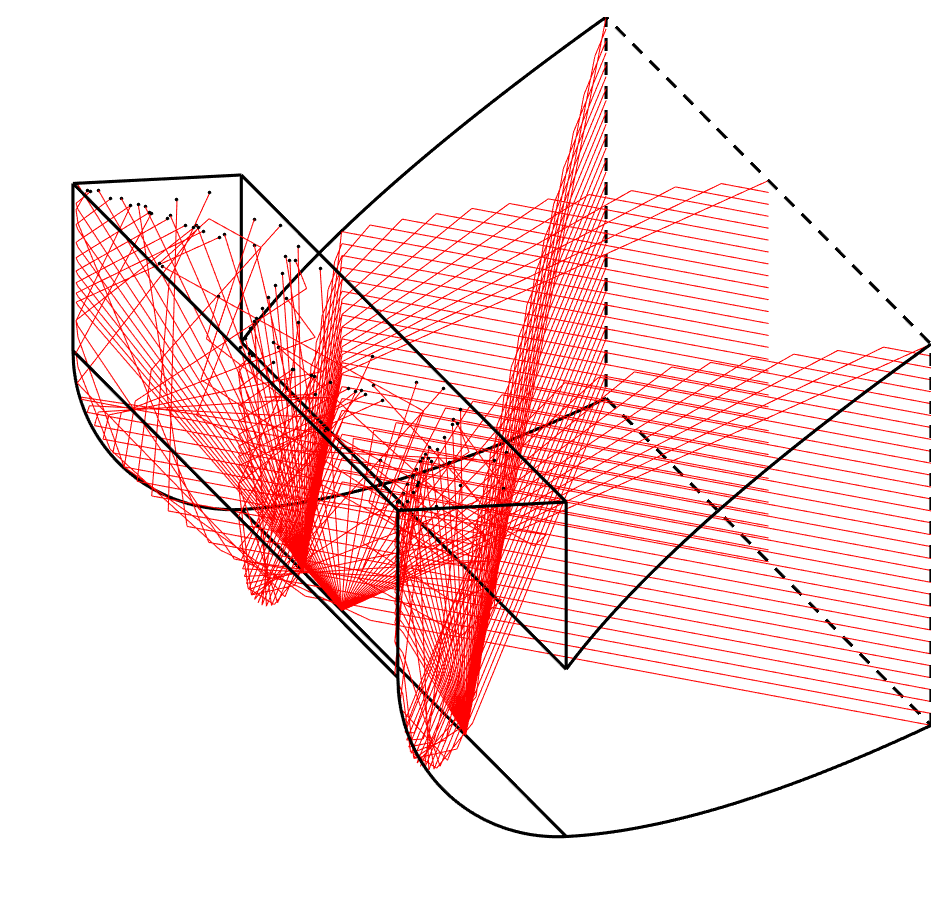
\includegraphics[width=0.95\columnwidth,height=5.5cm]{figs/3D-diagram-15.eps}
		\subcaption{3D RT diagram at $\rm{a_s = 15^o}$ and $\rm{\gamma_s = 70^o}$.}
	\end{minipage}
	\begin{minipage}{0.49\columnwidth}
		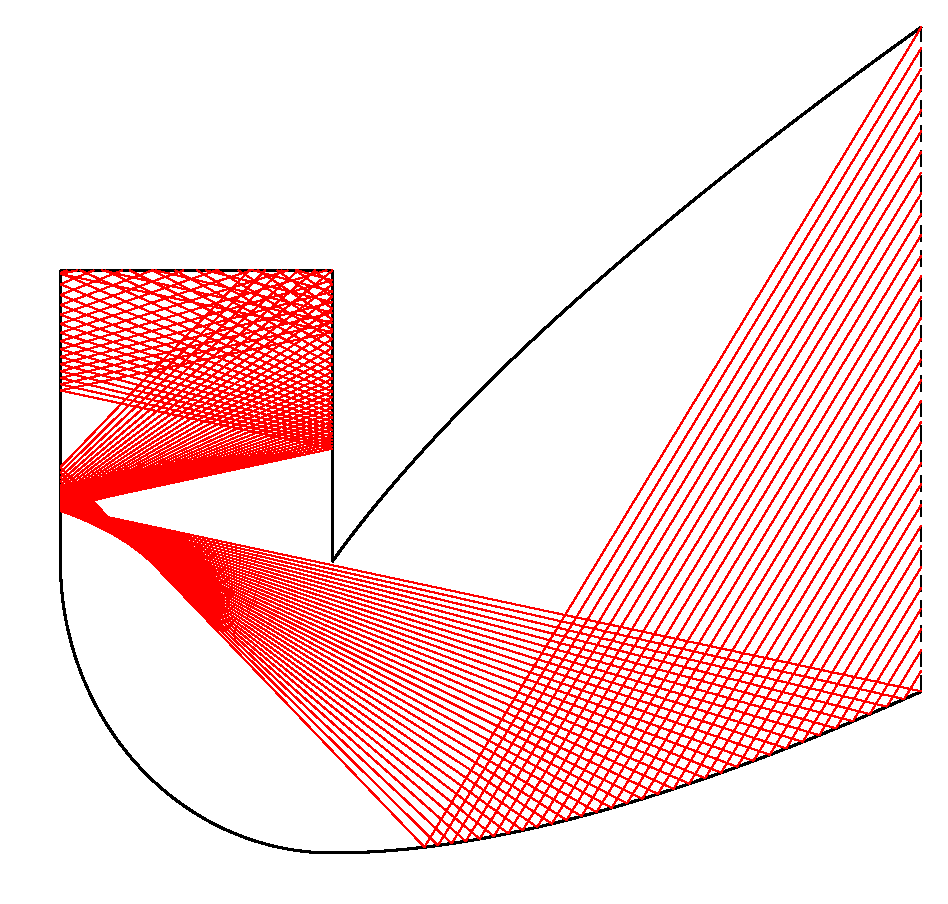
\includegraphics[width=0.90\columnwidth,height=5cm]{figs/2D-diagram-60.eps}
		\subcaption{2D RT diagram at $\rm{a_s = 60^o}$.}
		
		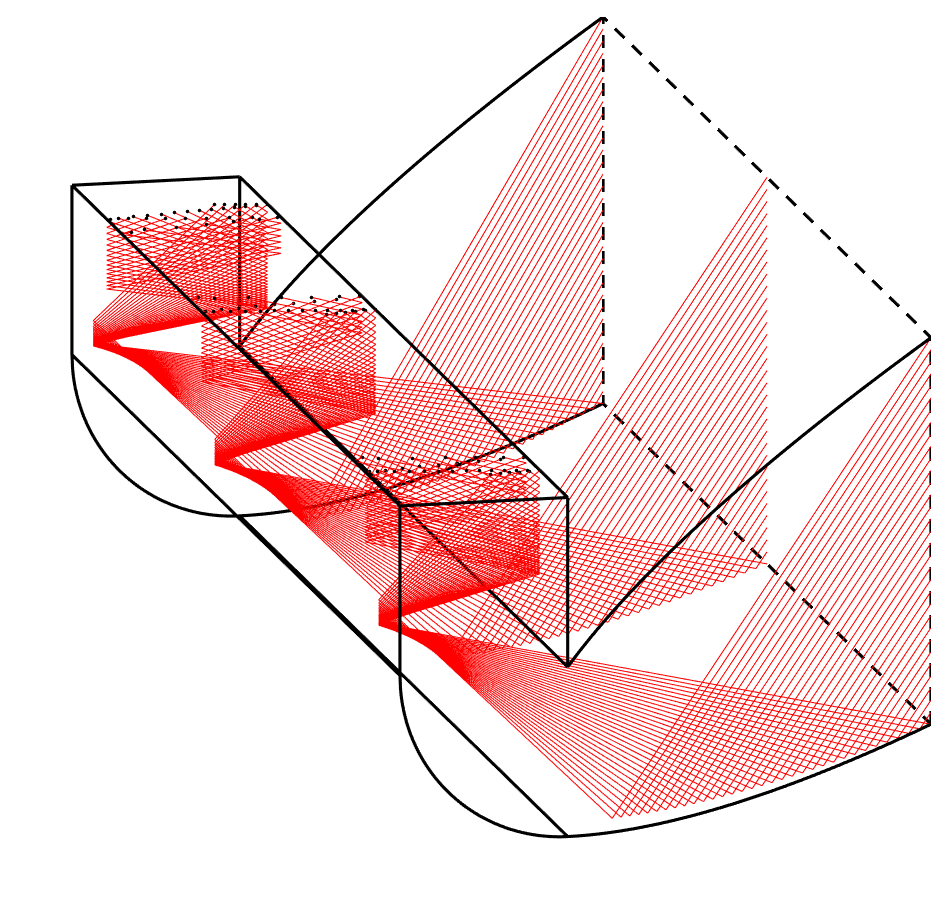
\includegraphics[width=0.95\columnwidth,height=5.5cm]{figs/3D-diagram-60.eps}
		\subcaption{3D RT diagram at $\rm{a_s = 60^o}$ and $\rm{\gamma_s = 10^o}$.}
		
	\end{minipage}
	\caption{Ray tracing diagrams in 2D and 3D.}
	\label{RT-diagram}
\end{figure}

%The glazing transmittance $\tau_{\rm{g}}$, calculated using equations described in \citet{Duffie2013}, is dependent of the inclination $\beta$, which affects the incident angle $\theta_{\rm{i}}$, defined as the angle between the incident solar ray and the normal to the glazing, is calculated by Eq. (\ref{incidence}):
%
%\begin{equation}
%\mathrm{\theta_i = {\cos ^{-1}}\left[ {\cos {a_s}\cos ({\gamma_s} - {\gamma_w})\sin \beta  + \sin {a_s}\cos \beta} \right]}
%\label{incidence}
%\end{equation}
%
%\noindent where $\gamma_{\rm{s}} = 0$ in the 2D analysis, and the concentrator azimuth angle $\gamma_{\rm{w}}$ is zero as the system is south facing.

The optical efficiency is defined as the ratio between the absorbed and the incident solar energy. Considering the number of reflections, glazing transmittance and absorber absorptance, it is calculated using Eq. (\ref{optical}) as a function of the reflectors' shape, the concentration ratio and the incident angle $\theta_{\rm i}$ from Eq. (\ref{incidence0}) (\cite{Sellami2013}):

\vspace{-0.75cm}
\begin{equation}
\mathrm{\eta_o = {\mathlarger{\sum\limits}_{\scriptscriptstyle i=1}^{\scriptscriptstyle \mathrm{N_{rays}}}{{\rho_{ref}^{{r_i}}}}}\tau_{glaz}\alpha_{abs}}
\label{optical}
\end{equation}

\noindent where $\rm{r_i}$ is the number of reflections of the solar ray i.

The effective concentration ratio ($\rm{C_{eff}}$), which is the product of the geometric concentration ratio and the optical efficiency, is given by Eq. (\ref{Ceff}). $\rm{C_{eff}}$ is useful to select shapes capable of enhancing both concentration of energy at the absorber and optical efficiency. All the optical outputs $\tau_{\rm {glaz}}$, $\eta_{\rm o}$ and $\rm{C_{eff}}$ can be calculated as averaged values to represent the whole period of operation for each particular concentrator. They were called $\tau_{\rm glaz,avg}$, $\eta_{\rm o,avg}$ and $\rm{C_{eff,avg}}$.

\vspace{-0.75cm}
\begin{equation}
\mathrm{C_{eff} = \eta_{\!_o}CR}
\label{Ceff}
\end{equation}

The collector's dimensions can also be related as dimensionless relative to the absorber width: $\rm{W^{*} = W_{col}/W_{abs}}$, $\rm{H^{*} = H_{col}/W_{abs}}$ and $\rm{L^{*} = L_{col}/W_{abs}}$. The dimensionless parameter A$^*$ was introduced to consider the reflector area relative to the absorber area, where:

\vspace{-0.75cm}
\begin{equation}
\mathrm{{A^*} = \frac{{{A_R}}}{{{A_{abs}}}} = \frac{{{W_r}}}{{{W_{abs}}}} + 2\frac{{{W^*}{H^*}}}{{{L^*}}}}
\label{reflectorarea}
\end{equation}

\noindent where $\rm{W_{ref}}$ (m) is the width of reflective material employed for a particular shape.

\section{Results and Discussion}

\subsection{Overview and collector specification}

This section was organised as follows:

\begin{itemize}[topsep=5pt,partopsep=0pt] \itemsep0pt
\item Design analysis of a standalone collector's geometry using the dimensionless parameters W$^{*}$, H$^{*}$ and A$^{*}$ at different parabolic shapes as a function of the truncation level (in terms of the geometric concentration ratio CR);
\item Optical performance considering the average values of optical efficiency $\rm{\eta_o}$ and effective concentration ratio $\rm{C_{eff}}$ at different shapes (in terms of $\theta_{\!_{\rm{P2}}}$) as a function of CR at a fixed absorber width, zero tertiary section height ($\rm{H_{TS} = 0}$) and $\rm{L_{col} = 10W_{abs}}$, 
\item Optical performance of two different geometries by varying the length;
\item Selection of the collector for further fabrication;
\item Evaluation of the cavity height on the optical efficiency and the energy distribution over the absorber;
\item Optical characterisation of the collector.
%\item Comparison of the combination of three different concentrator shapes on a fixed area of wall;
%\item Evaluation of the effect of the aperture size of the same collector at a fixed length;
%\item Analysis of different combinations in terms of aperture size at a fixed area of wall.
\end{itemize}

%\subsection{Collector specification}

An optical analysis was conducted for the solar air heating collector with the following specifications:

\begin{itemize} [topsep=5pt,partopsep=0pt] \itemsep0pt
    \item The absorber absorptance ($\alpha_{\rm{abs}}$) is 0.85;
    \item The reflector reflectance ($\rho_{\rm{ref}}$) is 0.95;
    \item A 4-mm thick low iron glass was employed with a refractive index of 1.526 and an extinction coefficient of 4 m$^{\!^{-1}}$. When the rays are perpendicular to the surface, the value of $\tau_{\rm{glaz}}$ is 0.90;
    \item The maximum truncation level was set to result in the minimum geometric concentration ratio of 2.0 regardless of the parabolic shape.
    \item The upper parabola axis angle was set to be coincident with the lowest solar altitude angle ($\theta_{\!_{\rm{P1}}}$ = 15$^{\circ}$);
    \item The range of lower parabola axis angles ($\theta_{\!_{\rm{P2}}}$) was between 44$^{\circ}$ and 61$^{\circ}$.
\end{itemize}

\subsection{Effect of the glazing inclination on the transmittance}

The glazing transmittance $\tau_{\rm{glaz}}$ varies in relation to the incident angle $\theta_{\rm{i}}$ as shown in Figure \ref{transm}. It was calculated using Eqs. (\ref{snell}), (\ref{rho_glaz}), (\ref{abs_glaz}) and (\ref{transmi}). The value of $\tau_{\rm{glaz}}$ is approximately 0.9 for incident angles lower than 40$^{\circ}$.

\Figure[scale=0.60,placement=!ht,label={transm},caption={Transmittance as function of the angle of incidence.}]{figs/transm.eps}

\newpage
The average transmittance calculated as a function of the glazing inclination is shown in Figure \ref{transmittance}. A maximum average transmittance is at \mbox{$\beta$ = 33$^{\circ}$} as 0.8907, thus is the inclination of which the glazing losses are minimum overall. Compared to the transmittance with the glazing placed vertically, there is a relative difference of 14\%. However, an inclination at $\beta$ = 33$^{\circ}$ brings practical difficulties, such as a high dust accumulation and rainwater over the glazing cover. For this reason, a steeper inclination was desirable, even though less solar energy is reaching the absorber. Therefore, \mbox{$\beta$ = 62$^{\circ}$} was chosen, where \mbox{$\tau_{\rm{g,avg}}$ = 0.8770}, more than 98\% of the maximum average transmittance.

\Figure[scale=0.60,placement=!ht,label={transmittance},caption={Average transmittance dependent on glazing inclination.}]{figs/transmittance.eps}

The results of instantaneous light transmittance against daytime is shown in Figure \ref{transm-time} for different glazing inclinations on 30$^{\rm th}$ June. The maximum transmittance profile is at $\beta$ = 33$^{\circ}$, whereas the one of inclination at the local latitude angle ($\beta$ = 53$^{\circ}$) and the one at $\beta$ = 62$^{\circ}$ do not present a significant difference. All three profiles are similar between 11:00 and 16:00 on this day. On the other hand, the vertical glazing profile shows the highest amount of solar reflection.

\Figure[scale=0.55,placement=!ht,label={transm-time},caption={Light transmittance throughout the day (30$^{\rm th}$ June).}]{figs/transm-time.eps}

\subsection{Design analysis of standalone collectors}

The dimensionless parameters $\rm{W^{*}}$ and $\rm{H^{*}}$ are presented by graphs in Figure \ref{size_region2}, where each graph corresponds to a particular shape. The maximum concentration ratio, obtained from the shape at $\theta_{\!_{\rm{P2}}} = 44^{\circ}$, was 2.98. $\rm{W^{*}}$ and $\rm{H^{*}}$ decrease as $\theta_{\!_{\rm{P2}}}$ increases for the same concentration ratio because the concentrator's acceptance angle is broader. For the same concentrator (fixed shape), the size increases when CR increases until its maximum aperture width, thus defining its maximum size (indicated by the dashed line in Figure \ref{size_region2}). The smallest concentrator has the shape of the narrowest acceptance angle ($\theta_{\!_{\rm{P2}}} = 44^{\circ}$) and the smallest concentration ratio (CR = 2.0) for being the most truncated ($\rm{W_{col} = 2.2W_{abs}}$ and $\rm{H_{col} = 2.2W_{abs}}$). In contrast, the largest concentrator has the narrowest acceptance angle but at the highest concentration ratio ($\rm{W_{col} = 7.3W_{abs}}$ and $\rm{H_{col} = 5.4W_{abs}}$). 

\Figure[scale=0.70,placement=!ht,label={size_region2},caption={Dimensionless parameters $\rm{W^{*}}$ and $\rm{H^{*}}$ matching particular CR for different shapes.}]{figs/size_region2.eps}

As shown in Figure \ref{reflector_region}, the dimensionless parameter $\rm{A^{*}}$ increases as the concentrator's size increases. Thus the graphs in Figures \ref{size_region2} and \ref{reflector_region} are similar. The reflector area varied from $\rm{5.4A_{abs}}$ for the smallest concentrator to nearly $\rm{24A_{abs}}$ for the largest one. Because this collector is an asymmetric compound parabolic concentrator, these graphs are similar to those found by \citet{Rabl1976} for symmetric concentrators.

\Figure[scale=0.70,placement=!ht,label={reflector_region},caption={Dimensionless parameter $\rm{A^{*}}$ matching particular CR for different shapes.}]{figs/reflector_region.eps}

%\Figure[scale=0.80,placement=!ht,label={size_region3},caption={Dimensionless parameter $\rm{A^{*}}$ matching particular CR for different shapes.}]{figs/size_region3.eps}

\subsection{Optical performance of standalone collectors}

\subsubsection{Optical performance by varying parabolic shape and truncation level}

The average optical efficiency as a function of CR for different shapes is shown in Figure \ref{eff_region2}. For concentrators of concentration ratio below 2.2, the shape of the highest optical efficiency is the one of $\theta_{\!_{\rm{P2}}} = 44^{\circ}$. For truncation levels resulting in a concentration ratio above 2.4, concentrators cannot accept a portion of direct solar radiation of solar altitude angles ($\rm{a_s}$) above 50$^{\circ}$, which is the reason why the graphs have decaying behaviours. The shape of $\theta_{\!_{\rm{P2}}} = 44^{\circ}$ and CR = 2.0 is the most efficient with $\rm{\eta_{o,avg} = 0.689}$ for being the smallest concentrator that accepts all direct solar radiation in the period of operation. The least efficient concentrator is the one of maximum CR ($\rm{\eta_{o,avg} = 0.432}$) because it requires more reflections for the solar rays to reach the absorber, and it does not accept direct solar radiation above $\rm{50^{\circ}}$ of $\rm{a_s}$, which is equivalent to 35\% of the period of operation.

\Figure[scale=0.67,placement=!ht,label={eff_region2},caption={$\rm{\eta_{o,avg}}$ matching particular CR for different shapes.}]{figs/eff_region2.eps}

The average effective concentration ratio $\rm{C_{eff,avg}}$ against CR and $\theta_{\!_{\rm{P2}}}$, is shown in Figure \ref{Ceff_region2}. Geometries of $\theta_{\!_{\rm{P2}}}$ below 56$^{\circ}$ have maximum values of $\rm{C_{eff,avg}}$ above 1.55 at each particular level of CR. After these conditions, the graphs dramatically drop as CR is increased due to the fall in optical efficiency, as discussed previously. The shape correspondent to the smallest $\rm{C_{eff,avg}}$ is the one of maximum CR ($\rm{C_{eff,avg} = 1.3}$) for being the least optically efficient; and the shape of maximum $\rm{C_{eff,avg}}$ is the one of $\theta_{\!_{\rm{P2}}} = 51^{\circ}$ and $\rm{CR = 2.5}$ although it is not able to accept direct solar radiation above $\rm{56^{\circ}}$ of $\rm{a_s}$. Concentrators of $\rm{CR = 2.0}$ are less effective in $\rm{C_{eff,avg}}$, despite being the most optically efficient concentrators.

\Figure[scale=0.65,placement=!ht,label={Ceff_region2},caption={$\rm{C_{eff,avg}}$ matching particular CR for different shapes.}]{figs/Ceff_region2.eps}

\subsubsection{Optical performance by varying concentrator length} 

The values of ${\rm \eta_{o,avg}}$ and $\rm{C_{eff,avg}}$ were calculated as a function of the dimensionless parameter $\rm{L^{*}}$ for two different concentrators: the most optically efficient (CR = 2.0) and one with the highest $\rm{C_{eff,avg}}$ (CR = 2.5). The results can be seen in Figure \ref{eff_length}. The values of ${\rm \eta_{o,avg}}$ assuming an infinite length, were 0.70 (CR = 2.0) and \mbox{0.662 (CR = 2.5)}. The end losses are higher for shorter concentrators due to more reflections. When the length is 3$\rm W_{abs}$, where $\rm \eta_{o,avg}$ is more than 95\% of the optical efficiency assuming infinite length. When $\rm{L_{col} = 10W_{abs}}$, the values of $\rm{\eta_{o,avg}}$ are more than 98\% of those assuming infinite length. Hence, a longer concentrator incurs fewer reflection losses at the ends, thus leading to higher optical efficiencies. However, the cost of additional reflective material and weight might not compensate for the little significant gain in energy collection.

\Figure[scale=0.75,placement=!ht,label={eff_length},caption={${\rm \eta_{o,avg}}$ matching particular $\rm{L^{*}}$ for two different concentrators.}]{figs/eff_length.eps}

\newpage
The end effect can be observed in more details when ${\rm \eta_{o,avg}}$ for four different length ratios are plotted against operation time. This is shown in Figure \ref{length_variance}, specifically on 30$^{\rm th}$ June for the smallest concentrator's performance (CR = 2.0). The end losses are higher in the beginning of the day due to higher values of the azimuth solar angles incurring in more reflections at the ends and therefore collectors collect less energy before noon, especially for shorter concentrators. 

\Figure[scale=0.65,placement=!ht,label={length_variance},caption={${\rm \eta_o}$ vs. time for a collector at different length ratios.}]{figs/length_variance.eps}

\subsection{Selection of the collector to be fabricated}

This topic used a criterion to select the collector's geometry to be fabricated for tests. The collector must accept solar radiation with $\rm{a_s}$ between 15$^{\circ}$ and 61$^{\circ}$. Once these limits were set, an initial design was sketched. The angles of both parabolic axes coincide with those limits, so all direct radiation within this range is accepted. From this design (shown in Figure \ref{collectors-61-50} in red), the absorber width achieved the maximum concentration ratio of 2.284. The actual aperture width ($\rm{W_{apt}}$) will be 0.33 m in order to have three collectors stacked on every metre of wall height. Hence, $\rm{W_{abs}}$ was found to be 0.145 m.

\Figure[scale=0.65,placement=!h,label={collectors-61-50},caption={Comparison between the collector at 61$^{\circ}$ of $\theta_{\!_{\rm{P2}}}$ (red) and the one at 50$^{\circ}$ (blue).}]{figs/collectors-61-50.eps}

As this collector is truncated, the range of angular acceptance may be broader than the limits previously defined. In order to validate this hypothesis, the ray tracing algorithm was used to check whether all the rays within this range were accepted. A graph of $\theta_{\rm{acc}}$ vs. ${\rm{a_s}}$ was plotted and shown in Figure \ref{acceptance}. The collector fully accepts direct radiation from 17$^{\circ}$ to 63$^{\circ}$ of ${\rm{a_s}}$, which exceeds the upper limit. Therefore, the collector's optical performance can be enhanced by further modifications to the reflectors. In this case, it was done by decreasing the lower parabola axis angle ($\theta_{\!_{\rm{P2}}}$). As this change in shape affects the number of reflections, $\rm{\eta_{\!_{o,avg}}}$ was calculated at different values of $\theta_{\!_{\rm{P2}}}$ and two graphs were plotted in Figure \ref{eff-alphaP2}. Although there is no significant gain in the average effective concentration ratio ($\rm{C_{eff,avg}}$ = 1.52) when both designs are compared, the parameter A* is reduced from 11.7 to 7.8, reducing the reflector area required by 33\%.

\Figure[scale=0.70,placement=!ht,label={acceptance},caption={Angular acceptance vs. solar altitude angle for the collector at 61$^{\circ}$ of $\alpha_{\!_{\rm{P2}}}$ (red) and the one at 50$^{\circ}$ of $\alpha_{\!_{\rm{P2}}}$ (blue).}]{figs/acceptance-graph.eps}

Furthermore, by ray tracing, the collector's angular acceptance at \mbox{$\theta_{\!_{\rm{P2}}}$ = 50$^{\circ}$} was calculated and shown in Figure \ref{acceptance} (in red). Although the full acceptance is up to 59$^{\circ}$, $\rm{\theta_{acc}}$ at 60$^{\circ}$ is above 90\%, which poorly influences the optical efficiency. From this analysis, the angles of the upper and lower parabola axes were 17$^{\rm o}$ and 50$^{\rm o}$, respectively. 

\Figure[scale=0.65,placement=!ht,label={eff-alphaP2},caption={Average optical efficiency {\itshape versus} lower parabola axis angle.}]{figs/eff-alphaP2.eps}

For the collector's length selection, the ray tracing technique was used to calculate the average optical efficiency as a function of this geometric parameter. The $\rm{\eta_{\!_{o,avg}}}$ versus $\rm{L_{col}}$ graph was plotted and shown in Figure \ref{eff-length}. For lengths above 2 m, there is little gain in efficiency (above 0.68), whereas, below this value, the reflection losses at the ends are higher, which worsens the optical performance. At $\rm{L_{col}}$ = 1.25 m, the collector's optical efficiency is 95\% of the maximum theoretical efficiency ($\rm{\eta_{\!_{o,avg}}}$ = 0.67). Therefore, this length was chosen for the collector's fabrication under optical consideration.

\Figure[scale=0.65,placement=!ht,label={eff-length},caption={Average optical efficiency {\itshape versus} collector's length.}]{figs/eff-length.eps}



\section{Optical characterisation of the proposed collector}

\subsection{Effect of the cavity height}

To understand the effect of the cavity height in the analysis, the average optical efficiency was calculated and shown in Figure \ref{opt-avg-hts} as a function of the tertiary section height. Adding a new reflective section will imply in more reflections, thus decreasing the average efficiency by approximately 3.5\%. To illustrate the effect of the tertiary section height, the collector's optical performance on 30$^{\rm th}$ June at three different heights was calculated and shown in Figure \ref{opt-eff-3hts}. The three profiles impose nearly the same efficiency from 09:00 to 10:30 and from 16:20 to 17:00. The highest difference is at 12:00, where $\eta_{\rm{o}}$ with no tertiary height is 0.71 and $\eta_{\rm{o}}$ at $\rm{H_{TS}}$ = $\rm{W_{abs}}$ is 0.61.

\Figure[scale=0.65,placement=!h,label={opt-avg-hts},caption={Average optical efficiency as function of the tertiary section height.}]{figs/opt-avg-hts.eps}

\Figure[scale=0.65,placement=!ht,label={opt-eff-3hts},caption={Optical efficiency profile for three tertiary section heights on 30$^{\rm th}$ June.}]{figs/opt-eff-3hts.eps}

Although the optical efficiency is reduced by the increase of the tertiary section height, the cavity distributes the incoming energy uniformly along the absorber surface. To demonstrate that in an example, the simulation results has the inputs: ${\rm{a_s}}$ at 54$^{\circ}$, $\gamma_{\rm{s}}$ at 0$^{\circ}$ and $\rm I_T$ at 1000~W/m$^2$. The results are shown in Figures \ref{Tertiary-hts0}, \ref{Tertiary-hts72} and \ref{Tertiary-hts145}. 

\newpage
From Figure \ref{Tertiary-hts0} with no tertiary section, a sharp peak in energy flux near the center of the absorber (close to 14 on the x-axis), with flux values exceeding 12500 W/m$^2$. The flux quickly diminishes from this central region, indicating that most of the energy is concentrated in a narrow band. All the energy is concentrated in 45 millimetres of width. 

\begin{figure}[ht!]
	\begin{minipage}{0.48\columnwidth}
		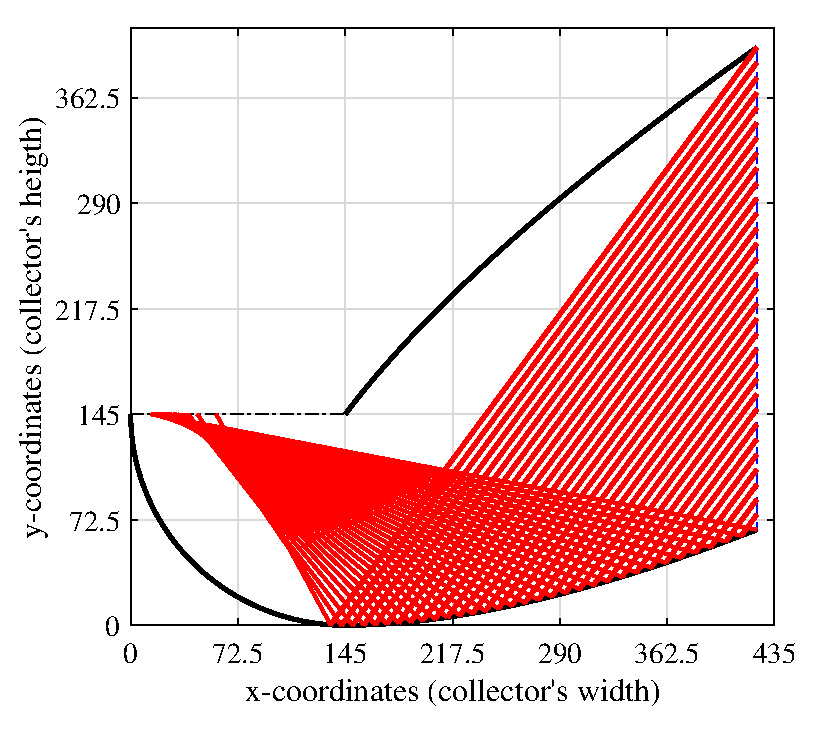
\includegraphics[scale=0.45]{figs/RT2D-hts0.eps}
		\subcaption{Ray tracing diagram (cross-section).}
		
	\end{minipage}
	\begin{minipage}{0.48\columnwidth}
		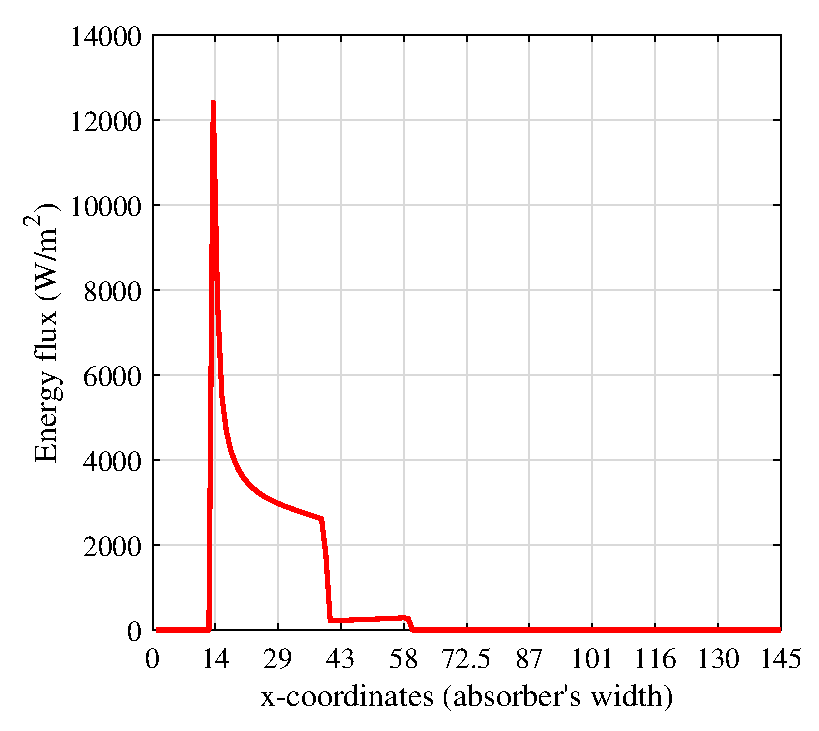
\includegraphics[scale=0.45]{figs/Energy2D-hts0.eps}
		%\\[-9mm]
		\subcaption{Energy flux distribution (cross-section).}
	\end{minipage}
	\\[3mm]
	\begin{minipage}{1.0\columnwidth}
		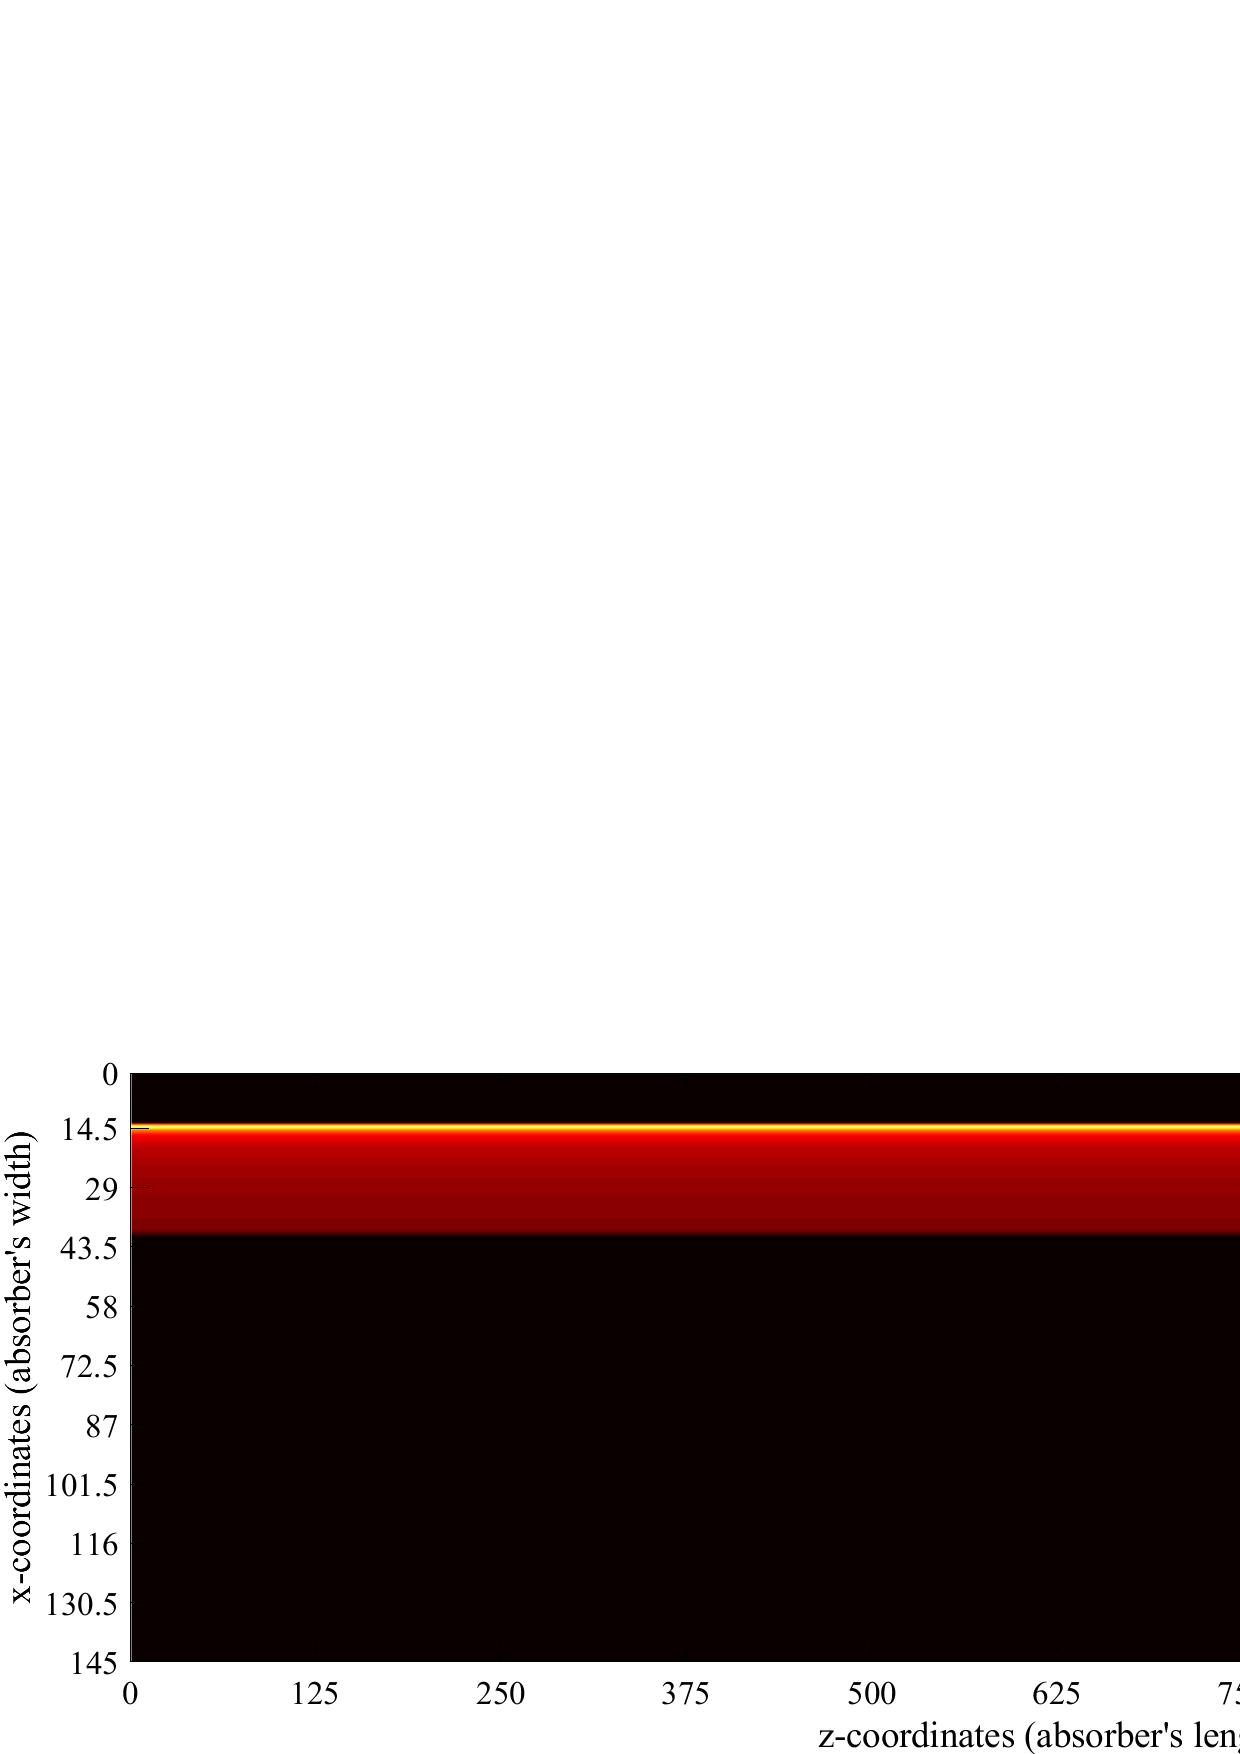
\includegraphics[scale=0.40]{figs/Energy3D-hts0.png}
		\subcaption{Energy flux distribution over the absorber surface (top view).}
	\end{minipage}
	
	\caption{Ray tracing diagram in 2D and energy flux distribution over the absorber width with no tertiary section.}
	\label{Tertiary-hts0}
\end{figure}

From Figure \ref{Tertiary-hts72} where the tertiary section height is half the width of the absorber, it can be observed that the energy flux peak is significantly reduced, reaching a maximum of 980 W/m$^2$) This represents a lower peak compared to the previous configuration shown in the earlier figure. Additionally, the decline in energy flux along the absorber width is more gradual, which implies in a smoother distribution of solar energy. It is evident that the peak region is concentrated within a narrow band of just 6 mm in width, highlighting a localised area of high intensity.

\begin{figure}[ht!]
	\begin{minipage}{0.48\columnwidth}
		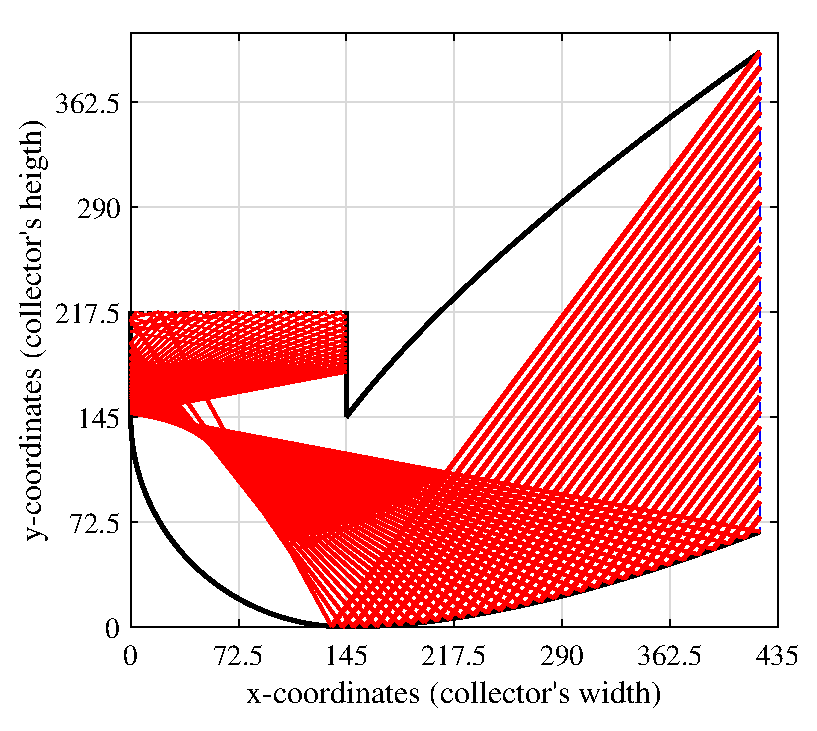
\includegraphics[scale=0.45]{figs/RT2D-hts72.eps}
		\subcaption{Ray tracing diagram (cross-section).}
		
	\end{minipage}
	\begin{minipage}{0.48\columnwidth}
		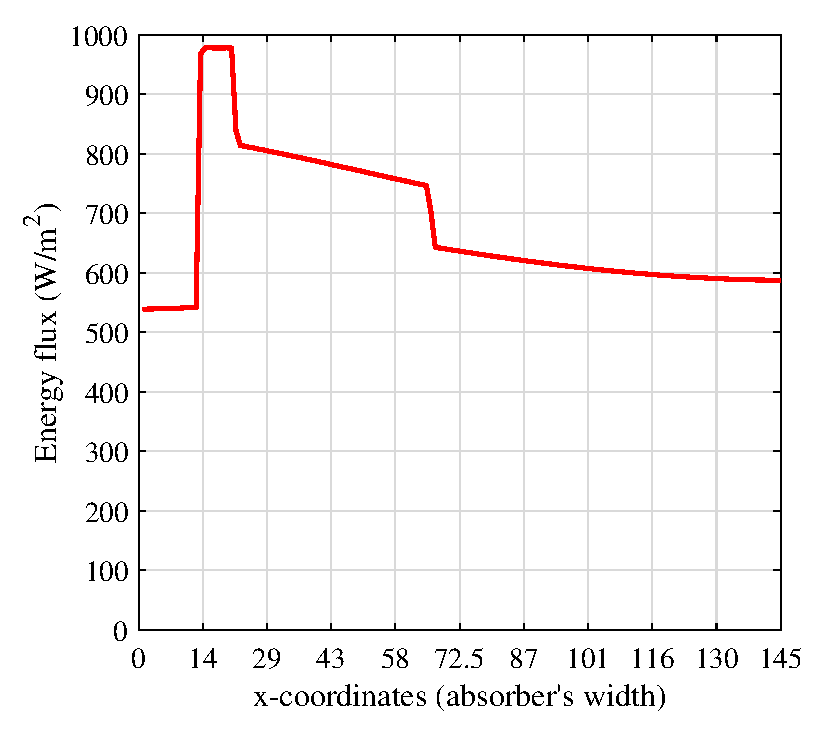
\includegraphics[scale=0.45]{figs/Energy2D-hts72.eps}
		%\\[-9mm]
		\subcaption{Energy flux distribution (cross-section).}
	\end{minipage}
	\\[3mm]
	\begin{minipage}{1.0\columnwidth}
		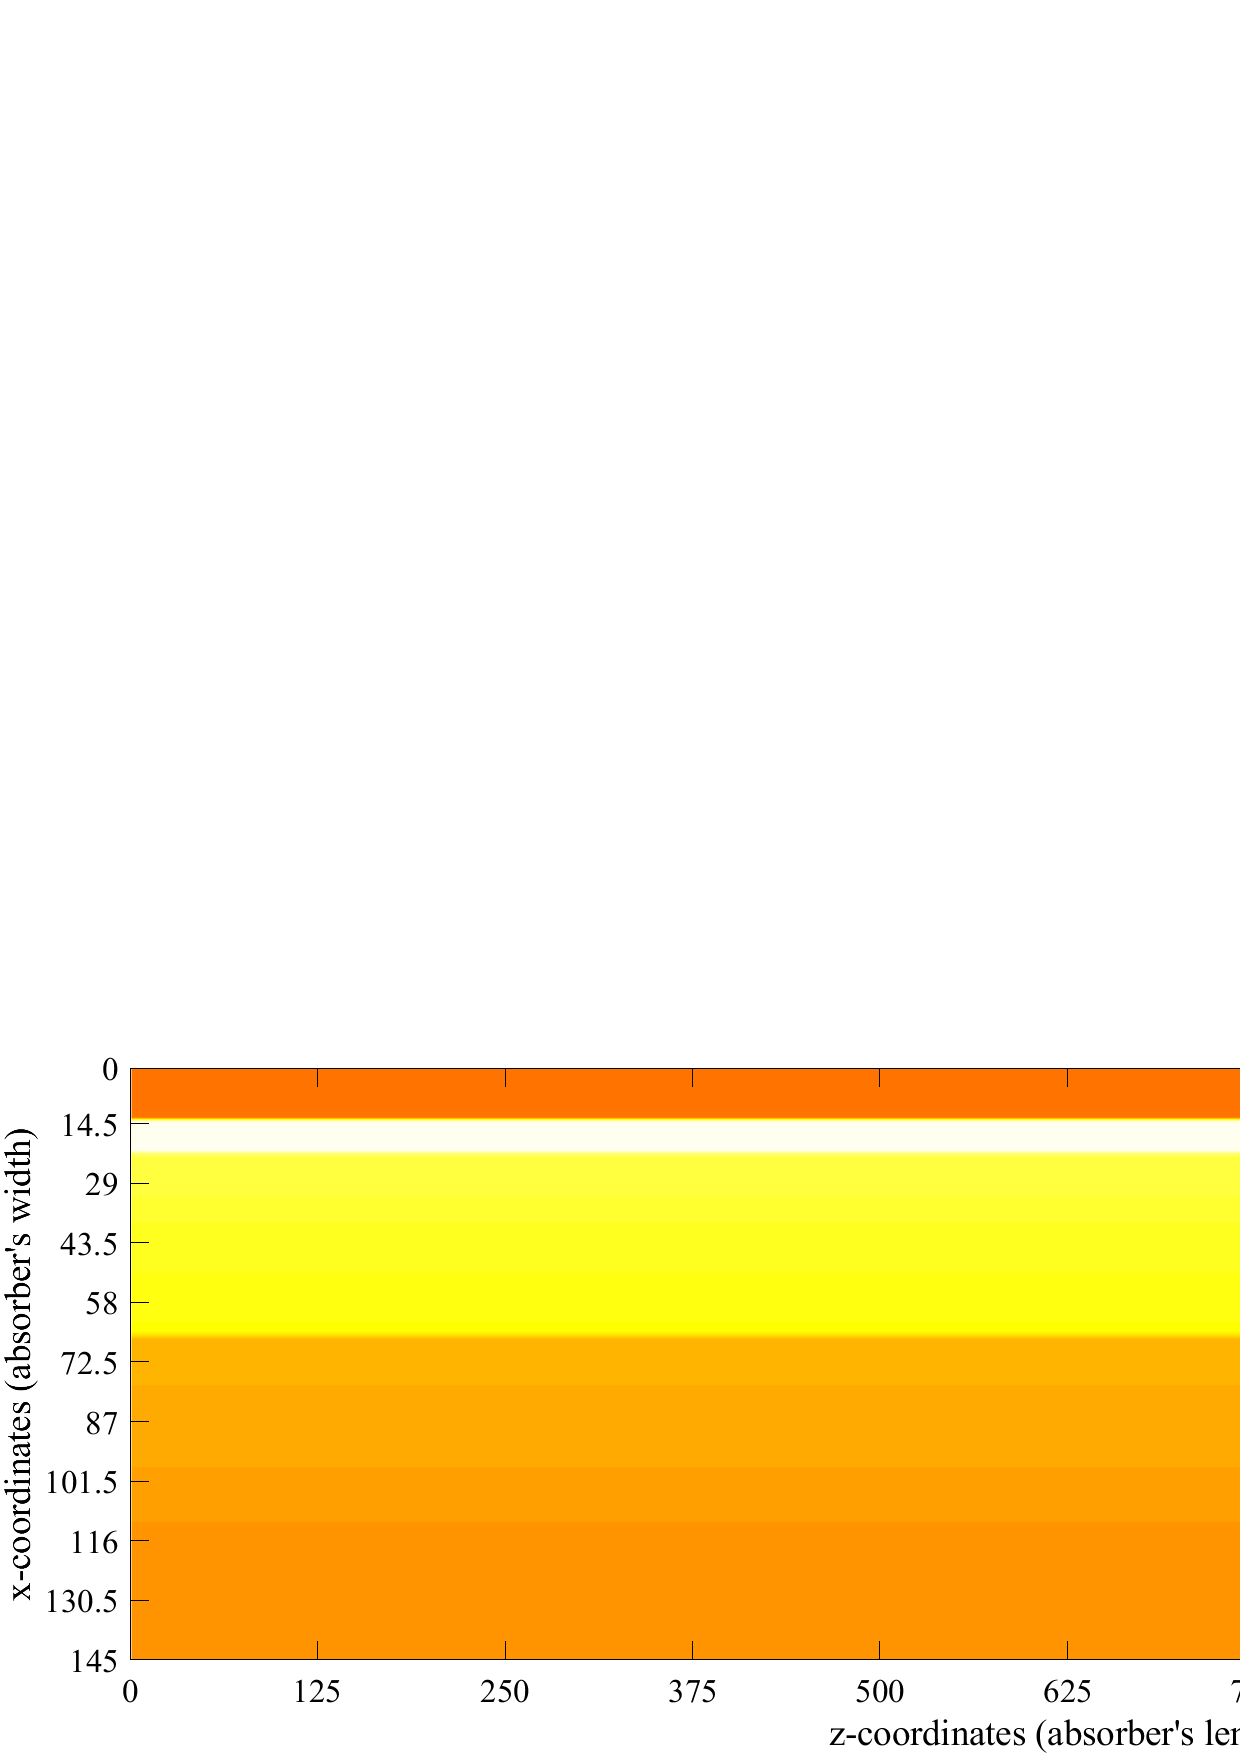
\includegraphics[scale=0.40]{figs/Energy3D-hts72.png}
		\subcaption{Energy flux distribution over the absorber surface (top view).}
	\end{minipage}
	
	\caption{Ray tracing diagram in 2D and energy flux distribution over the absorber width with tertiary section height of 72.5 mm.}
	\label{Tertiary-hts72}
\end{figure}

\newpage
From Figure \ref{Tertiary-hts145}, illustrates a scenario where the energy flux is more evenly distributed across the surface of the absorber. The maximum energy flux observed is 740 W/m$^2$ which spans across half of the absorber width. This broader distribution of energy is advantageous for improving the uniformity of heat transfer across the absorber. While the tertiary section contributes to this more balanced energy dispersion, it also leads to higher reflection losses. Despite this trade-off, the cavity height was set to be 0.145 m.

\begin{figure}[ht!]
	\begin{minipage}{0.48\columnwidth}
		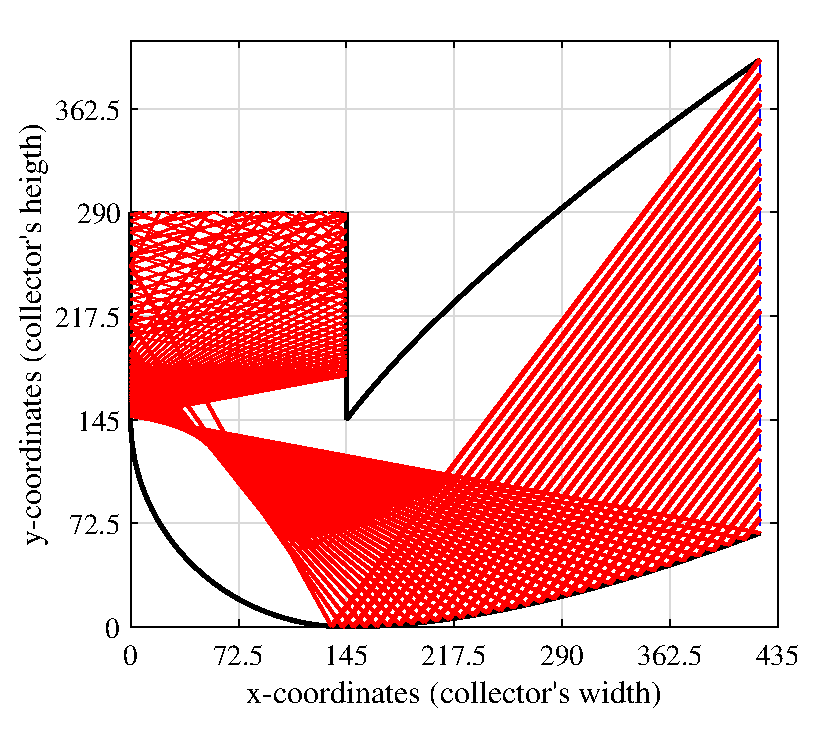
\includegraphics[scale=0.45]{figs/RT2D-hts145.eps}
		\subcaption{Ray tracing diagram (cross-section).}
		
	\end{minipage}
	\begin{minipage}{0.48\columnwidth}
		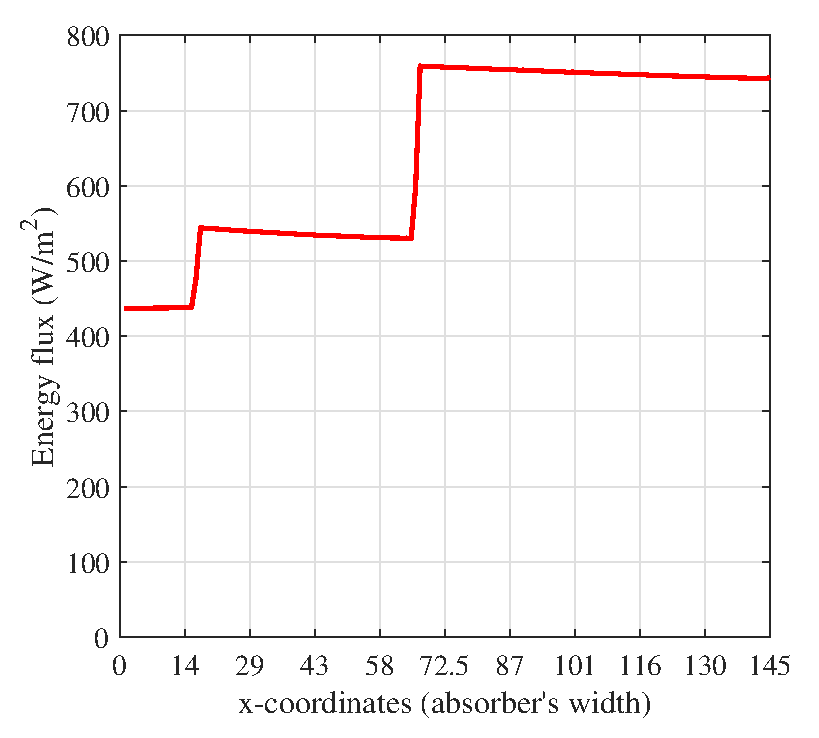
\includegraphics[scale=0.45]{figs/Energy2D-hts145.eps}
		%\\[-9mm]
		\subcaption{Energy flux distribution (cross-section).}
	\end{minipage}
	\\[3mm]
	\begin{minipage}{1.0\columnwidth}
		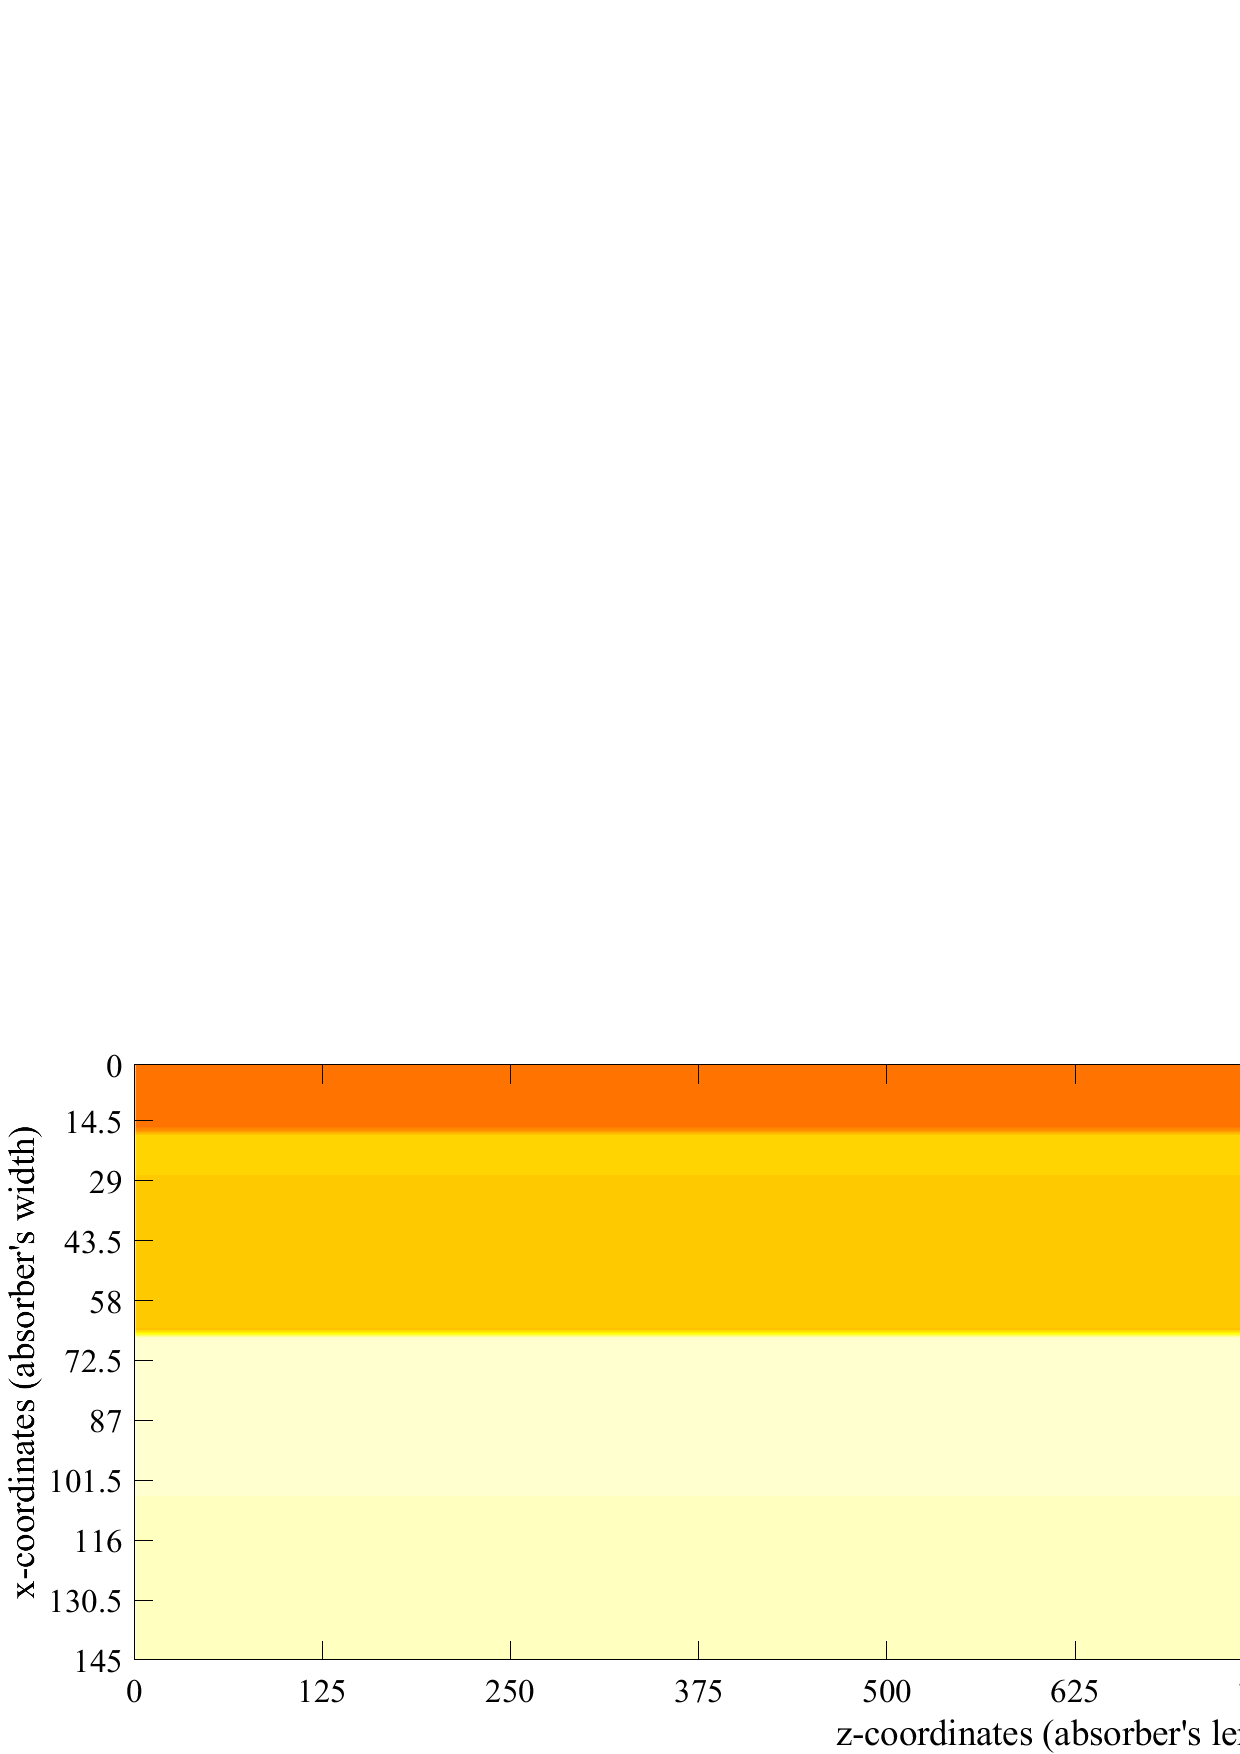
\includegraphics[scale=0.40]{figs/Energy3D-hts145.png}
		\subcaption{Energy flux distribution over the absorber surface (top view).}
	\end{minipage}
	
	\caption{Ray tracing diagram in 2D and energy flux distribution over the absorber width with tertiary section height of 145 mm.}
	\label{Tertiary-hts145}
\end{figure}

\subsection{Optical efficiency profile}

After the optical analysis, the concentrator's design was defined, as shown in Figure \ref{collector3p} and the main geometric parameters are summarised in Table \ref{optics_parameters}. The glazing inclination has been set at $\beta$ = 62$^{\circ}$ for practical reasons related to its width. 

\Figure[scale=0.70,placement=!ht,label={collector3p},caption={Cross section of the collector's final design.},frame]{figs/collector3p.eps}

\begin{table}[!ht]
	\caption{Geometric parameters of the concentrator to be fabricated.}
	\centering
	\begin{tabular}{p{1.75cm}p{4.5cm}p{2.0cm}}
		\hline \\[-10pt]
		Symbol & Geometric parameter & Value \\ [2pt]
		\hline \\[-12pt]
		$\rm{L_{col}}$ & Concentrator length & 1.25 m \\ [2pt]
		
		$\rm{H_{col}}$ & Concentrator height & 0.40 m \\ [2pt]
		
		$\rm{W_{col}}$ & Concentrator depth & 0.43 m \\ [2pt]
		
		$\rm{W_{abs}}$ & Absorber width & 0.145 m \\ [2pt]
		
		$\rm{A_{abs}}$ & Absorber area & 0.18 m$^2$ \\ [2pt]
		
		$\rm{W_{glaz}}$ & Glazing width & 0.27 m \\ [2pt]
		
		$\rm{A_{glaz}}$ & Glazing area & 0.34 m$^2$ \\ [2pt]
		
		$\beta$ & Glazing inclination & 62$^{\circ}$ \\ [2pt]
		
		$\rm{W_{apt}}$ & Aperture width & 0.33 m \\ [2pt]
		
		$\rm{A_{apt}}$ & Aperture area & 0.41 m$^2$ \\ [2pt]
		
		$\rm{H_{\!_{TS}}}$ & Cavity height & 0.145 m \\ [2pt]
		
		$\rm{CR}$ & Concentration ratio & 2.28 \\ [2pt]
		
		$\rm{A_{ref}}$ & Reflector area & 2 m$^2$ \\
		
		\hline 
	\end{tabular}
	\label{optics_parameters}
\end{table}

\newpage
Figure \ref{opt-eff-time} shows the optical profile as a function of daytime and date during the summer. The efficiency peaks between 12:00 and 14:00 during midday, as indicated by the red regions corresponding to the highest values (around 0.69). This period aligns with the solar noon, where solar altitude angle is highest, and the collector operates at maximum  optical performance. In contrast, the blue areas show that the optical efficiency diminishes in the early morning (09:00 -- 10:00) and late afternoon (16:00 -- 17:00). These lower values are likely due to reduced solar angles and optical losses due to higher reflections. Seasonal variations are also evident, with the highest efficiency observed near the summer solstice (21/06). During this time, the longer daylight hours and higher solar angles can contribute to more consistent and elevated optical efficiency throughout the day. As the dates progress toward the autumn equinox (21/09), there is a noticeable decline in efficiency, reflected by an expansion of the lower-efficiency regions (blue and green zones). This decline can be attributed to shorter daylight hours and lower solar angles as the season transitions, which increase optical losses and reduce the system's overall performance. The average optical efficiency for direct radiation of this collector is 0.67. To determine the energy an airflow absorbs, conducting experimental studies or using a reliable energy balance calculation is essential.

\Figure[scale=0.62,placement=!ht,label={opt-eff-time},caption={Optical efficiency profile throughout the whole period of operation.}]{figs/opt-eff-time.eps}

\section{Chapter Summary}

% The selection of an air heater concentrator with the absorber horizontally facing downwards aims to concentrate solar thermal energy inside the cavity and suppress heat losses. With the assistance of a ray tracing technique in 3D, an optical analysis has been undertaken to evaluate its optical efficiency considering factors as: glazing transmittance, truncation level, length and tertiary section height. The results show that there is a maximum value of optical efficiency for a particular parabolic reflector shape and a maximum value of glazing transmittance at different inclinations. It was also concluded that the energy distributed along the absorber area is more uniform with a tertiary section rather than without it even though the optical losses are higher. The effect of the tertiary section on the collector's performance needs to be further assessed, via thermal modelling and outdoor experiments. Finally, a solar concentrator design was proposed through optical analysis, and its 3D optical profile over time was presented at the end of the chapter. The proposed air heater concentrator is able to absorb in average 67\% of direct solar radiation during most part of the day in the period evaluated.

The chapter presented the design, development, and analysis of a solar air heating concentrator that integrates an inverted absorber with Asymmetric Compound Parabolic Concentrators (IACPC). This system was designed to enhance optical efficiency and reduce heat losses. The concentrator employs geometric configurations, including parabolic, circular, and straight reflectors, combined with a glazing cover to retain solar radiation and protect the system from environmental conditions. A tertiary section is added to improve energy distribution across the absorber, a feature that trades some optical efficiency for better heat transfer uniformity. The study uses 3D ray tracing simulations to evaluate the system's optical performance, focusing on factors such as glazing inclination, truncation levels, and reflector geometry. The results demonstrate an average optical efficiency of 67\% during the system's operating hours, highlighting its capability to harness direct solar radiation effectively. Key design optimisations include setting the concentration ratio at 2.28 and ensuring a compact structure with a length of 1.25 m and a height of 0.4 m. This makes the system suitable for practical applications, including integration into building fa\c{c}ades.

